% Created 2020-01-06 Mon 14:34
% Intended LaTeX compiler: pdflatex
\documentclass[dvipdfmx,10pt]{article}
\usepackage[utf8]{inputenc}
\usepackage[T1]{fontenc}
\usepackage{graphicx}
\usepackage{grffile}
\usepackage{longtable}
\usepackage{wrapfig}
\usepackage{rotating}
\usepackage[normalem]{ulem}
\usepackage{amsmath}
\usepackage{textcomp}
\usepackage{amssymb}
\usepackage{capt-of}
\usepackage{hyperref}
%% Margin
%% \usepackage[margin=1.5cm]{geometry}
\usepackage[top=1.5cm, bottom=1.5cm, left=1.5cm, right=1.5cm, headsep=4pt]{geometry}
%% \addtolength{\topmargin}{0.3cm}
%% \addtolength{\textheight}{1.75in}
%% Math
\usepackage{amsmath}
\usepackage{amssymb}
\usepackage{wasysym}
%% Allow new page within align
\allowdisplaybreaks
\usepackage{cancel}
% % Code
\usepackage{listings}
\usepackage{courier}
\lstset{basicstyle=\footnotesize\ttfamily, breaklines=true, frame=single}
\usepackage[cache=false]{minted}
\usemintedstyle{vs}
%% Graphics
\usepackage{graphicx}
\usepackage{grffile}
%% DAG
\usepackage{tikz}
\usetikzlibrary{positioning,shapes.geometric}
%% Date
\usepackage[yyyymmdd]{datetime}
\renewcommand{\dateseparator}{--}
%% Header
\usepackage{fancyhdr}
\pagestyle{fancy}
\fancyhf{} % Erase first to supress section names
\fancyhead[L]{Kazuki Yoshida} % LEFT
\fancyhead[C]{} % CENTER
\fancyhead[R]{\today} % RIGHT
\fancyfoot[C]{\thepage}
%% \fancyfoot[R]{Page \thepage\ of \pageref{LastPage}}
%% Section font size
\usepackage{sectsty}
\sectionfont{\small}
\subsectionfont{\small}
\subsubsectionfont{\small}
%% Section numbering
%% http://tex.stackexchange.com/questions/3177/how-to-change-the-numbering-of-part-chapter-section-to-alphabetical-r
%% \renewcommand\thesection{\alph{section}}
%% \renewcommand\thesubsection{\thesection.\arabic{subsection}}
%% \renewcommand{\thesubsubsection}{\thesubsection.\alph{subsubsection}}
%%
%% http://tex.stackexchange.com/questions/40067/numbering-sections-with-sequential-integers
%% \usepackage{chngcntr}
%% \counterwithout{subsection}{section}
%% enumerate
\usepackage{enumerate}
%% double space
%% \usepackage{setspace}
%% \linespread{2}
%% Paragraph Indentation
\usepackage{indentfirst}
\setlength{\parindent}{0em}
%% Spacing after headings
%% http://tex.stackexchange.com/questions/53338/reducing-spacing-after-headings
\usepackage{titlesec}
\titlespacing      \section{0pt}{12pt plus 4pt minus 2pt}{0pt plus 2pt minus 2pt}
\titlespacing   \subsection{0pt}{12pt plus 4pt minus 2pt}{0pt plus 2pt minus 2pt}
\titlespacing\subsubsection{0pt}{12pt plus 4pt minus 2pt}{0pt plus 2pt minus 2pt}
%% Fix figures and tables by [H]
\usepackage{float}
%% Allow URL embedding
\usepackage{url}
\usepackage{fontawesome}
\input{\string~/.emacs.d/misc/GrandMacros}
\author{Kazuki Yoshida \\ \\ \faTwitter \href{https://twitter.com/kaz\_yos}{@kaz\_yos} \faGithub \href{https://github.com/kaz-yos/}{kaz-yos}}
\date{\today\\}
\title{Equivalence of G-formula and IPTW}
\hypersetup{
 pdfauthor={Kazuki Yoshida \\ \\ \faTwitter \href{https://twitter.com/kaz\_yos}{@kaz\_yos} \faGithub \href{https://github.com/kaz-yos/}{kaz-yos}},
 pdftitle={Equivalence of G-formula and IPTW},
 pdfkeywords={},
 pdfsubject={},
 pdfcreator={Emacs 26.3 (Org mode 9.3.1)}, 
 pdflang={English}}
\begin{document}

\maketitle
\sloppy
\section{INTRODUCTION}
\label{sec:org2c6a77f}
\subsection{IPTW and G-formula}
\label{sec:org504c3f4}
\begin{itemize}
\item Here we will demonstrate the equivalence of the IPTW \cite{robinsMarginalStructuralModels2000} and the \emph{g}-formula \cite{robinsNewApproachCausal1986} given saturated models.
\item Special thanks to \href{https://twitter.com/edwardhkennedy/status/1119305663564472320}{@edwardhkennedy}!
\end{itemize}

\subsection{Notations}
\label{sec:org6ed8118}
\begin{align*}
  Y &: \text{Outcome measured at the end of the study}\\
  Y^{a_{0}} &: \text{Counterfactual outcome with intervention at time 0 only}\\
  Y^{a_{0},a_{1}} &: \text{Counterfactual outcome with intervention at time 0 and 1}\\
  L_{0} &: \text{Baseline covariates}\\
  A_{0} &: \text{Baseline treatment assignment}\\
  L_{1} &: \text{Post-baseline covariates}\\
  A_{1} &: \text{Post-baseline treatment assignment}\\
\end{align*}

Here we assume both \(L_{t}\) and \(A_{t}\) are discrete.

\subsection{Causal structure}
\label{sec:orgf52156e}
\begin{enumerate}
\item Original DAG
\label{sec:org4e6a470}
\begin{center}
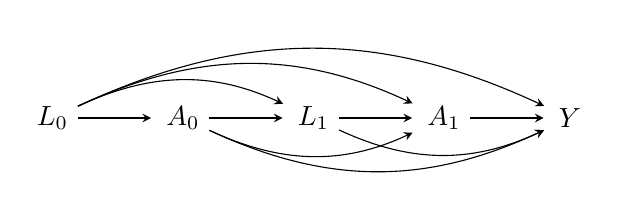
\begin{tikzpicture}[%
  ->,
  shorten >=2pt,
  >=stealth,
  node distance=1cm,
  pil/.style={
    ->,
    thick,
    shorten =2pt,}
  ]
  %% Nodes
  \node (L0) {$L_{0}$};
  \node[right = 1cm of L0] (A0) {$A_{0}$};
  \node[right = 1cm of A0] (L1) {$L_{1}$};
  \node[right = 1cm of L1] (A1) {$A_{1}$};
  \node[right = 1cm of A1] (Y) {$Y$};
  %% Edges
  \draw[->] (L0) to (A0);
  \draw[->] (L0) to [out=25,in=155] (L1);
  \draw[->] (L0) to [out=25,in=155] (A1);
  \draw[->] (L0) to [out=25,in=155] (Y);
  \draw[->] (A0) to (L1);
  \draw[->] (A0) to [out=-25,in=-155] (A1);
  \draw[->] (A0) to [out=-25,in=-155] (Y);
  \draw[->] (L1) to (A1);
  \draw[->] (L1) to [out=-25,in=-155] (Y);
  \draw[->] (A1) to (Y);
\end{tikzpicture}
\end{center}

\item Single time point intervention SWIG
\label{sec:orgb98c3c9}
\begin{center}
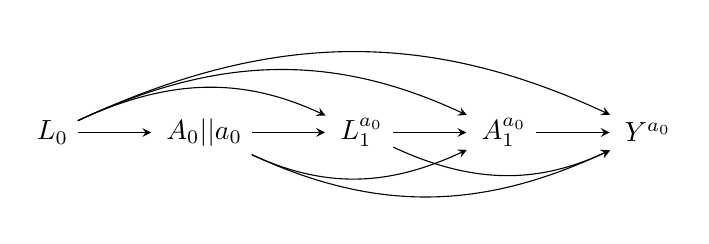
\begin{tikzpicture}[%
  ->,
  shorten >=2pt,
  >=stealth,
  node distance=1cm,
  pil/.style={
    ->,
    thick,
    shorten =2pt,}
  ]
  %% Nodes
  \node (L0) {$L_{0}$};
  \node[right = 1cm of L0] (A0) {$A_{0}||a_{0}$};
  \node[right = 1cm of A0] (L1) {$L_{1}^{a_{0}}$};
  \node[right = 1cm of L1] (A1) {$A_{1}^{a_{0}}$};
  \node[right = 1cm of A1] (Y) {$Y^{a_{0}}$};
  %% Edges
  \draw[->] (L0) to (A0);
  \draw[->] (L0) to [out=25,in=155] (L1);
  \draw[->] (L0) to [out=25,in=155] (A1);
  \draw[->] (L0) to [out=25,in=155] (Y);
  \draw[->] (A0) to (L1);
  \draw[->] (A0) to [out=-25,in=-155] (A1);
  \draw[->] (A0) to [out=-25,in=-155] (Y);
  \draw[->] (L1) to (A1);
  \draw[->] (L1) to [out=-25,in=-155] (Y);
  \draw[->] (A1) to (Y);
\end{tikzpicture}
\end{center}

\item Two time point intervention SWIG
\label{sec:org60f07b7}
\begin{center}
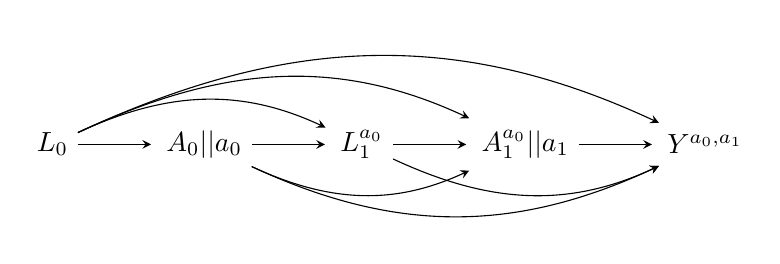
\begin{tikzpicture}[%
  ->,
  shorten >=2pt,
  >=stealth,
  node distance=1cm,
  pil/.style={
    ->,
    thick,
    shorten =2pt,}
  ]
  %% Nodes
  \node (L0) {$L_{0}$};
  \node[right = 1cm of L0] (A0) {$A_{0}||a_{0}$};
  \node[right = 1cm of A0] (L1) {$L_{1}^{a_{0}}$};
  \node[right = 1cm of L1] (A1) {$A_{1}^{a_{0}}||a_{1}$};
  \node[right = 1cm of A1] (Y) {$Y^{a_{0},a_{1}}$};
  %% Edges
  \draw[->] (L0) to (A0);
  \draw[->] (L0) to [out=25,in=155] (L1);
  \draw[->] (L0) to [out=25,in=155] (A1);
  \draw[->] (L0) to [out=25,in=155] (Y);
  \draw[->] (A0) to (L1);
  \draw[->] (A0) to [out=-25,in=-155] (A1);
  \draw[->] (A0) to [out=-25,in=-155] (Y);
  \draw[->] (L1) to (A1);
  \draw[->] (L1) to [out=-25,in=-155] (Y);
  \draw[->] (A1) to (Y);
\end{tikzpicture}
\end{center}
\end{enumerate}


\section{Single time point strategy}
\label{sec:org75a5ac0}
\subsection{Identifiability Conditions}
\label{sec:org6698a64}
\begin{itemize}
\item We will follow the terminologies in \cite{hernanCausalInference2019} (Chapter 3).
\item 1. \textbf{Consistency}: the values of treatment under comparison correspond to well-defined interventions that, in turn, correspond to the versions of treatment in the data
\end{itemize}
\begin{center}
\(Y_{i} = Y_{i}^{a_{0}}\) if \(A_{0i} = a_{0}\) for all \(a_{0}\)
\end{center}
\begin{itemize}
\item 2. \textbf{Exchangeability}: the conditional probability of receiving every value of treatment, though not decided by the investigators, depends only on the measured covariates
\end{itemize}
\begin{center}
\(A_{0} \ind Y^{a_{0}} | L_{0}\) for all \(a_{0}\)
\end{center}
\begin{itemize}
\item 3. \textbf{Positivity}: the conditional probability of receiving every value of treatment is greater than zero, i.e., positive
\end{itemize}
\begin{center}
\(f(A_{0} = a_{0} | L_{0} = l_{0}) > 0\) for all \(a_{0},l_{0}\) where \(f(L_{0} = l_{0}) > 0\)
\end{center}

\subsection{G-formula}
\label{sec:org068b635}
This follows the Technical Point 2.3 in \cite{hernanCausalInference2019}.
\begin{align*}
  &~~~\text{By iterative expectation}\\
  E[Y^{a_{0}}]
  &= E[E[Y^{a_{0}} | L_{0}]]\\
  &~~~\text{By conditional exchangeability: } Y^{a_{0}} \ind A_{0} | L_{0}\\
  &= E[E[Y^{a_{0}} | A_{0}, L_{0}]]\\
  &~~~\text{By exchangeability, }E[Y^{a_{0}} | A_{0}, L_{0}] = E[Y^{a_{0}} | A_{0} = a_{0}, L_{0}]\\
  &= E[E[Y^{a_{0}} | A_{0} = a_{0}, L_{0}]]\\
  &~~~\text{By consistency}\\
  &= E[E[Y | A_{0} = a_{0}, L_{0}]]\\
  &~~~\text{Make outer expectation explicit sum}\\
  &= \sum_{l_{0}} E[Y | A_{0} = a_{0}, L_{0} = l_{0}] f(L_{0} = l_{0})\\
  &= \text{Conditional mean averaged over $L_{0}$}\\
\end{align*}

\subsection{IPTW}
\label{sec:org42b4f3d}
This follows the Technical Point 2.3 in \cite{hernanCausalInference2019}.
\begin{align*}
  &~~~\text{By iterative expectation}\\
  E[Y^{a_{0}}]
  &= E[E[Y^{a_{0}} | L_{0}]]\\
  &~~~\text{Insert a carefully-crafted expression that is 1.}\\
  &= E \left[ \frac{f(A_{0}=a_{0} | L_{0})}{f(A_{0}=a_{0} | L_{0})} E[Y^{a_{0}} | L_{0}] \right]\\
  &~~~\text{Using probability = expectation of indicator}\\
  &= E \left[ \frac{E[I(A_{0}=a_{0}) | L_{0}]}{f(A_{0}=a_{0} | L_{0})} E[Y^{a_{0}} | L_{0}] \right]\\
  &~~~\text{Conditional exchangeability: } Y^{a_{0}} \ind A_{0} | L_{0}\\
  &~~~\text{This allows merging the two inner expectations.}\\
  &= E \left[ \frac{1}{f(A_{0}=a_{0} | L_{0})} E[I(A_{0}=a_{0})Y^{a_{0}} | L_{0}] \right]\\
  &~~~\text{By stability, } g(L_{0}) = E[g(L_{0}) | L_{0}].\\
  &~~~\text{i.e., a function of $L_{0}$ only (IPTW expression) can go into $E[\cdot | L_{0}]$}\\
  &= E \left[ E \left[ \frac{1}{f(A_{0}=a_{0} | L_{0})} I(A_{0}=a_{0})Y^{a_{0}} \bigg| L_{0} \right] \right]\\
  &~~~\text{Reversing iterative expectation (tower property)}\\
  &= E \left[ \frac{1}{f(A_{0}=a_{0} | L_{0})} I(A_{0}=a_{0})Y^{a_{0}} \right]\\
  &~~~\text{By consistency, }I(A_{0}=a_{0})Y^{a_{0}} = I(A_{0}=a_{0})Y = Y \text{ for } A_{0} = a_{0}.\\
  &~~~\text{Also, }I(A_{0}=a_{0})Y^{a_{0}} = 0 = I(A_{0}=a_{0})Y \text{ for } A_{0} \ne a_{0}.\\
  &~~~\text{Thus, }I(A_{0}=a_{0})Y^{a_{0}} = I(A_{0}=a_{0})Y \text{ regardless of } A_{0}.\\
  &= E \left[ \frac{1}{f(A_{0}=a_{0} | L_{0})} I(A_{0}=a_{0})Y \right]\\
  &= \text{IPTW mean of $Y$ for group $A_{0} = a_{0}$}\\
\end{align*}

\begin{itemize}
\item Law of Total Expectation (Iterative Expectation): \url{https://en.wikipedia.org/wiki/Law\_of\_total\_expectation}
\item Stability and Tower Property: \url{https://en.wikipedia.org/wiki/Conditional\_expectation\#Basic\_properties}
\item Indicator function: \url{https://www.statlect.com/fundamentals-of-probability/indicator-functions}
\item Expectation of product of random variables: \url{https://en.wikipedia.org/wiki/Product\_distribution\#Expectation\_of\_product\_of\_random\_variables}
\end{itemize}

\section{Multiple time point strategy}
\label{sec:orgdf55f13}
\subsection{Identifiability Conditions}
\label{sec:org310e42f}
\begin{itemize}
\item We will follow the terminologies in \cite{hernanCausalInference2019} (Chapter 19, Technical Point 19.2).
\item 1. \textbf{Consistency}: the values of treatment under comparison correspond to well-defined interventions that, in turn, correspond to the versions of treatment in the data
\end{itemize}
\begin{center}
\(Y_{i} = Y_{i}^{a_{0},a_{1}}\) if \(A_{0i} = a_{0}, A_{1i} = a_{1}\) for all \(a_{0},a_{1}\)
\end{center}
\begin{itemize}
\item 2. \textbf{Exchangeability}: the conditional probability of receiving every value of treatment, though not decided by the investigators, depends only on the measured covariates
\end{itemize}
\begin{center}
\(A_{0} \ind Y^{a_{0},a_{1}} | L_{0}\) for all \(a_{0},a_{1}\)

\(A_{1} \ind Y^{a_{0},a_{1}} | L_{1},A_{0}=a_{0},L_{0}\) for all \(a_{0},a_{1}\)
\end{center}
\begin{itemize}
\item 3. \textbf{Positivity}: the conditional probability of receiving every value of treatment is greater than zero, i.e., positive
\end{itemize}
\begin{center}
\(f(A_{0} = a_{0} | L_{0} = l_{0}) > 0\) for all \(a_{0},l_{0}\) where \(f(L_{0} = l_{0}) > 0\)

\(f(A_{1} = a_{1} | L_{1} = l_{1}, A_{0} = a_{0}, L_{0} = l_{0}) > 0\) for all \(a_{1},l_{1},a_{0},l_{0}\) where \(f(L_{1} = l_{1}, A_{0} = a_{0}, L_{0} = l_{0}) > 0\)
\end{center}

\subsection{G-formula}
\label{sec:org1f416cd}
This follows the Technical Point 2.3 in \cite{hernanCausalInference2019}.
\begin{align*}
  &~~~\text{By iterative expectation}\\
  E[Y^{a_{0},a_{1}}]
  &= E[E[Y^{a_{0},a_{1}} | L_{0}]]\\
  &~~~\text{By conditional exchangeability: } Y^{a_{0},a_{1}} \ind A_{0} | L_{0}\\
  &= E[E[Y^{a_{0},a_{1}} | A_{0}, L_{0}]]\\
  &~~~\text{By exchangeability, }E[Y^{a_{0},a_{1}} | A_{0}, L_{0}] = E[Y^{a_{0},a_{1}} | A_{0} = a_{0}, L_{0}]\\
  &= E[E[Y^{a_{0},a_{1}} | A_{0} = a_{0}, L_{0}]]\\
  &~~~\text{By iterative expectation}\\
  &= E[E[ E[Y^{a_{0},a_{1}} | L_{1}, A_{0} = a_{0}, L_{0}] | A_{0} = a_{0}, L_{0}]]\\
  &~~~\text{By conditional exchangeability: } Y^{a_{0},a_{1}} \ind A_{1} | L_{1},A_{0},L_{0}\\
  &= E[E[ E[Y^{a_{0},a_{1}} | A_{1}, L_{1}, A_{0} = a_{0}, L_{0}] | A_{0} = a_{0}, L_{0}]]\\
  &~~~\text{By exchangeability, }\\
  &~~~E[Y^{a_{0},a_{1}} | A_{1}, L_{1}, A_{0} = a_{0}, L_{0}] = E[Y^{a_{0},a_{1}} | A_{1} = a_{1}, L_{1}, A_{0} = a_{0}, L_{0}]\\
  &= E[E[ E[Y^{a_{0},a_{1}} | A_{1} = a_{1}, L_{1}, A_{0} = a_{0}, L_{0}] | A_{0} = a_{0}, L_{0}]]\\
  &~~~\text{By consistency}\\
  &= E[E[ E[Y | A_{1} = a_{1}, L_{1}, A_{0} = a_{0}, L_{0}] | A_{0} = a_{0}, L_{0}]]\\
  &~~~\text{Make outer expectations explicit sums}\\
  &= \sum_{l_{0}} \sum_{l_{1}}
    E[Y | A_{1} = a_{1}, L_{1} = l_{1}, A_{0} = a_{0}, L_{0} = l_{0}]\\
  &~~~\times f(L_{1} = l_{1} | A_{0} = a_{0}, L_{0} = l_{0}) f(L_{0} = l_{0})\\
\end{align*}

\subsection{IPTW}
\label{sec:orgdd14d2d}
This follows the Technical Point 2.3 in \cite{hernanCausalInference2019} and an input from \href{https://twitter.com/edwardhkennedy/status/1119305663564472320}{@edwardhkennedy}.
\begin{align*}
  &~~~\text{By iterative expectation}\\
  E\left[Y^{a_{0},a_{1}}\right]
  &= E\left[E\left[Y^{a_{0},a_{1}} | L_{0}\right]\right]\\
  &~~~\text{Insert a carefully-crafted expression that is 1.}\\
  &= E\left[\frac{f(A_{0}=a_{0} | L_{0})}{f(A_{0}=a_{0} | L_{0})} E\left[Y^{a_{0},a_{1}} | L_{0}\right]\right]\\
  &~~~\text{Using probability = expectation of indicator}\\
  &= E\left[\frac{E \left[ I(A_{0}=a_{0}) | L_{0} \right]}{f(A_{0}=a_{0} | L_{0})} E\left[Y^{a_{0},a_{1}} | L_{0}\right]\right]\\
  &~~~\text{By conditional exchangeability: } Y^{a_{0},a_{1}} \ind A_{0} | L_{0}\\
  &~~~\text{Thus, product of expectation = expectation of product}\\
  &= E\left[\frac{1}{f(A_{0}=a_{0} | L_{0})} E\left[I(A_{0}=a_{0})Y^{a_{0},a_{1}} | L_{0}\right]\right]\\
  &~~~\text{Law of total expectation}\\
  &= E\left[
    \frac{1}{f(A_{0}=a_{0} | L_{0})} E\left[I(A_{0}=a_{0})Y^{a_{0},a_{1}} | A_{0}=a_{0}, L_{0}\right]
    \right.\\
  &~~~~~~~~+\left.
    \frac{1}{f(A_{0}=a_{0} | L_{0})} E\left[I(A_{0}=a_{0})Y^{a_{0},a_{1}} | A_{0}\ne a_{0}, L_{0}\right]
    \right]\\
  &~~~\text{Indicator in second inner expectation = 0}\\
  &= E\left[\frac{1}{f(A_{0}=a_{0} | L_{0})} E\left[I(A_{0}=a_{0})Y^{a_{0},a_{1}} | A_{0} = a_{0}, L_{0}\right]\right]\\
  &~~~\text{By iterative expectation}\\
  &= E\left[\frac{1}{f(A_{0}=a_{0} | L_{0})} E\left[E\left[I(A_{0}=a_{0})Y^{a_{0},a_{1}} |L_{1}, A_{0} = a_{0}, L_{0}\right] | A_{0} = a_{0}, L_{0}\right]\right]\\
  &~~~\text{Insert a carefully-crafted expression that is 1.}\\
  &= E\left[\frac{1}{f(A_{0}=a_{0} | L_{0})}\times\right.\\
  &~~~~~~~\left.
    E\left[ \frac{f(A_{1}=a_{1} | L_{1}, A_{0} = a_{0}, L_{0})}{f(A_{1}=a_{1} | L_{1}, A_{0} = a_{0}, L_{0})}
    E\left[I(A_{0}=a_{0})Y^{a_{0},a_{1}} |L_{1}, A_{0} = a_{0}, L_{0}\right] \bigg| A_{0} = a_{0}, L_{0}\right]\right]\\
  &~~~\text{Using probability = expectation of indicator}\\
  &= E\left[\frac{1}{f(A_{0}=a_{0} | L_{0})}\times\right.\\
  &~~~~~~~\left.
    E\left[ \frac{E \left[ I(A_{1}=a_{1}) | L_{1}, A_{0} = a_{0}, L_{0} \right]}{f(A_{1}=a_{1} | L_{1}, A_{0} = a_{0}, L_{0})}
    E\left[I(A_{0}=a_{0})Y^{a_{0},a_{1}} |L_{1}, A_{0} = a_{0}, L_{0}\right] \bigg| A_{0} = a_{0}, L_{0}\right]\right]\\
  &~~~\text{By conditional exchangeability: } Y^{a_{0},a_{1}} \ind A_{1} | L_{1},A_{0} = a_{0},L_{0}\\
  &~~~\text{Thus, product of expectation = expectation of product}\\
  &= E\left[\frac{1}{f(A_{0}=a_{0} | L_{0})}\times\right.\\
  &~~~~~~~\left.
    E\left[ \frac{E\left[I(A_{0}=a_{0})I(A_{1}=a_{1})Y^{a_{0},a_{1}} |L_{1}, A_{0} = a_{0}, L_{0}\right]}{f(A_{1}=a_{1} | L_{1}, A_{0} = a_{0}, L_{0})}
     \bigg| A_{0} = a_{0}, L_{0}\right]\right]\\
  &~~~\text{IPTW at time 1 is a constant given }L_{1}, A_{0} = a_{0}, L_{0}\\
  &= E\left[\frac{1}{f(A_{0}=a_{0} | L_{0})}\times\right.\\
  &~~~~~~~\left.
    E\left[
    E\left[\frac{I(A_{0}=a_{0})I(A_{1}=a_{1})Y^{a_{0},a_{1}}}{f(A_{1}=a_{1} | L_{1}, A_{0} = a_{0}, L_{0})} \bigg|L_{1}, A_{0} = a_{0}, L_{0}\right]
     \bigg| A_{0} = a_{0}, L_{0}\right]\right]\\
  &~~~\text{Reverse iterative expectation (tower property)}\\
  &= E\left[\frac{1}{f(A_{0}=a_{0} | L_{0})}
    E\left[
    \frac{I(A_{0}=a_{0})I(A_{1}=a_{1})Y^{a_{0},a_{1}}}{f(A_{1}=a_{1} | L_{1}, A_{0} = a_{0}, L_{0})}
    \bigg| A_{0} = a_{0}, L_{0}\right]\right]\\
  &~~~\text{Add a second term that is zero by indicator }I(A_{0}=a_{0})\\
  &= E\left[\frac{1}{f(A_{0}=a_{0} | L_{0})}
    E\left[\frac{I(A_{0}=a_{0})I(A_{1}=a_{1})Y^{a_{0},a_{1}}}{f(A_{1}=a_{1} | L_{1}, A_{0} = a_{0}, L_{0})} \bigg| A_{0} = a_{0}, L_{0}\right]
    \right.\\
  &~~~~~~~\left. +\frac{1}{f(A_{0}=a_{0} | L_{0})}
  E\left[\frac{I(A_{0}=a_{0})I(A_{1}=a_{1})Y^{a_{0},a_{1}}}{f(A_{1}=a_{1} | L_{1}, A_{0} = a_{0}, L_{0})} \bigg| A_{0} \ne a_{0}, L_{0}\right]
\right]\\
  &~~~\text{Thus, we can drop conditioning on $A_{0}$.}\\
  &= E\left[\frac{1}{f(A_{0}=a_{0} | L_{0})}
    E\left[
    \frac{I(A_{0}=a_{0})I(A_{1}=a_{1})Y^{a_{0},a_{1}}}{f(A_{1}=a_{1} | L_{1}, A_{0} = a_{0}, L_{0})}
    \bigg| L_{0}\right]\right]\\
  &~~~\text{IPTW at time 0 is a constant given }L_{0}\\
  &= E\left[
    E\left[
    \frac{I(A_{0}=a_{0})I(A_{1}=a_{1})Y^{a_{0},a_{1}}}{f(A_{0}=a_{0} | L_{0})f(A_{1}=a_{1} | L_{1}, A_{0} = a_{0}, L_{0})}
    \bigg| L_{0}\right]\right]\\
  &~~~\text{Reverse iterative expectation (tower property)}\\
  &= E\left[
    \frac{I(A_{0}=a_{0})I(A_{1}=a_{1})Y^{a_{0},a_{1}}}{f(A_{0}=a_{0} | L_{0})f(A_{1}=a_{1} | L_{1}, A_{0} = a_{0}, L_{0})}
    \right]\\
  &~~~\text{By consistency and presence of indicators}\\
  &~~~I(A_{0}=a_{0})I(A_{1}=a_{1})Y^{a_{0},a_{1}} = I(A_{0}=a_{0})I(A_{1}=a_{1})Y \text{ for all }A_{0},A_{1}\\
  &~~~\text{That is, consistency where $A_{0}=a_{0},A_{1}=a_{1}$, otherwise both sides are zeros.}\\
  &= E\left[
    \frac{I(A_{0}=a_{0})I(A_{1}=a_{1})Y}{f(A_{0}=a_{0} | L_{0})f(A_{1}=a_{1} | L_{1}, A_{0} = a_{0}, L_{0})}
    \right]\\
  &= \text{IPTW mean of $Y$ for group $A_{0} = a_{0}, A_{1} = a_{1}$}\\
\end{align*}

\section{Bibliography Part}
\label{sec:orgd857011}
\subsection{Bibliography}
\label{sec:org1a18317}
\renewcommand{\section}[2]{}

\bibliographystyle{apalike}
\bibliography{../../../../.emacs.d/misc/zotero}
\end{document}